\documentclass{article}
\usepackage{amsmath}

\usepackage[letterpaper]{geometry}

\usepackage{booktabs}
\usepackage{textcomp}
\usepackage{float}
\usepackage{graphicx}
\graphicspath{{./doc_imgs/}}
\usepackage[utf8]{inputenc}

\usepackage{indentfirst}

\addtolength{\topmargin}{-1.00in}
\addtolength{\textheight}{1.5in}


\begin{document}

\title{RoseLap v4: Lap Time and Point Simulation}
\author{Thaddeus Hughes}

\maketitle

\begin{abstract}
RoseGPE is a student design competition team at Rose-Hulman that competes in the Formula SAE competitions, typically at the Lincoln and Michigan events. RoseGPE is driven by students learning and gaining work experience, and does this by aiming to score high at competition. To do this, the team builds a new prototype vehicle every year.

The competition is historically composed of 3/8 'static' events (cost judging, design judging, business case judging) and 5/8 'dynamic' events (acceleration, skidpad, autocross, endurance, and fuel economy)- meaning there are many facets to earning points and doing well.

Lap Time Simulation can be utilized to determine the configuration of vehicle which can produce the most points at competition. Determining points outcome from the acceleration, skipad, autocross, and endurance events is largely straightforward.
\end{abstract}

\section{Problem Introduction}
Lap Time Simulation is a numerical process. The general premise is to apply simplistic physics models to a car traveling over a small, finite stretch of track with given curvature to determine the next vehicle state. By stitching these segments together, with a strategy of when to brake, shift, or otherwise drive the vehicle, the operation of a racecar under idealized conditions can be simulated with useful accuracy.

These simulation results can be useful, potentially, to assist a driver in training for a track. They can also be useful and motivating for an engineer to understand how a vehicle drives around the track in detail, monitoring grip. The real value, however, lies in the ability to vary parameters and see how they impact lap times (and fuel consumption).

These lap times can be used with point formulas and other data to determine the overall point limit of a car at a particular competition.

\section{Pre-Processing and Input Data}
Blah blah dxfs and YAML

\subsection{Tire Data Fitting}
As discussed in the 'Tires' section, tire models used in RoseLap v4 are rather simplistic, but are more sophisticated than the constant COF presumed in v3 and prior. To determine the four parameters, some fitting must be done.

Tire data is obtained through physical testing. We use the data purchased from the Milliken Tire Test Consortium (TTC). This contains drive-brake and combined loading, with sweeps over various conditions.

With the python tool provided in \texttt{tire\_utility}, we examine the relationship between lateral and longitudinal force as it relates to normal force.

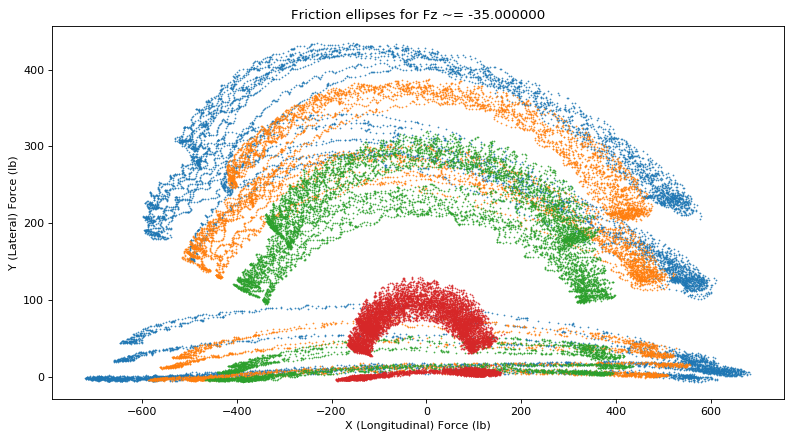
\includegraphics[width=\textwidth]{fric_ellipses.png}

The multiple colors indicate different normal forces. While imperfect, it is easy to see how fitting an ellipse to this would provide a reasonable model of tire behavior.

The first step is to determine the bins to which tire data vertical loads fall into. This is accomplished with a histogram.

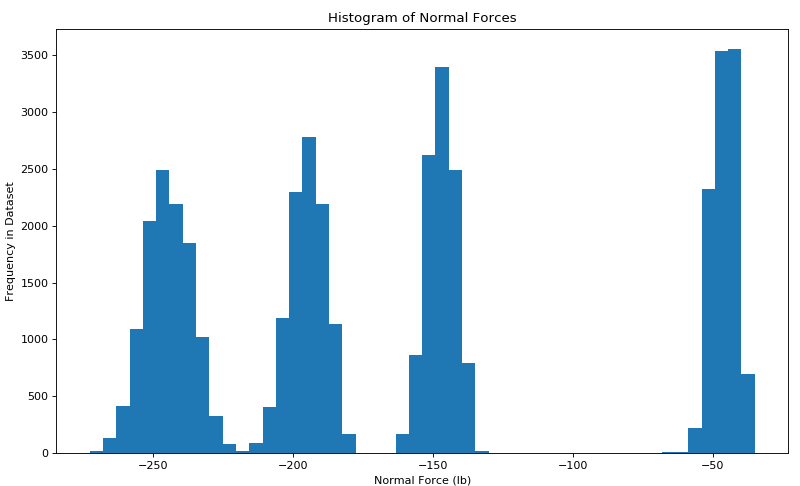
\includegraphics[width=\textwidth]{fric_hist.png}

Then, the data is analyzed in the Fz-Fx space and the Fz-Fy space. Outliers (outside of a 2-sigma confidence interval) are rejected. From here, the maximum grip datapoints from each bin are selected, and a linear regression is ran to fit these points.

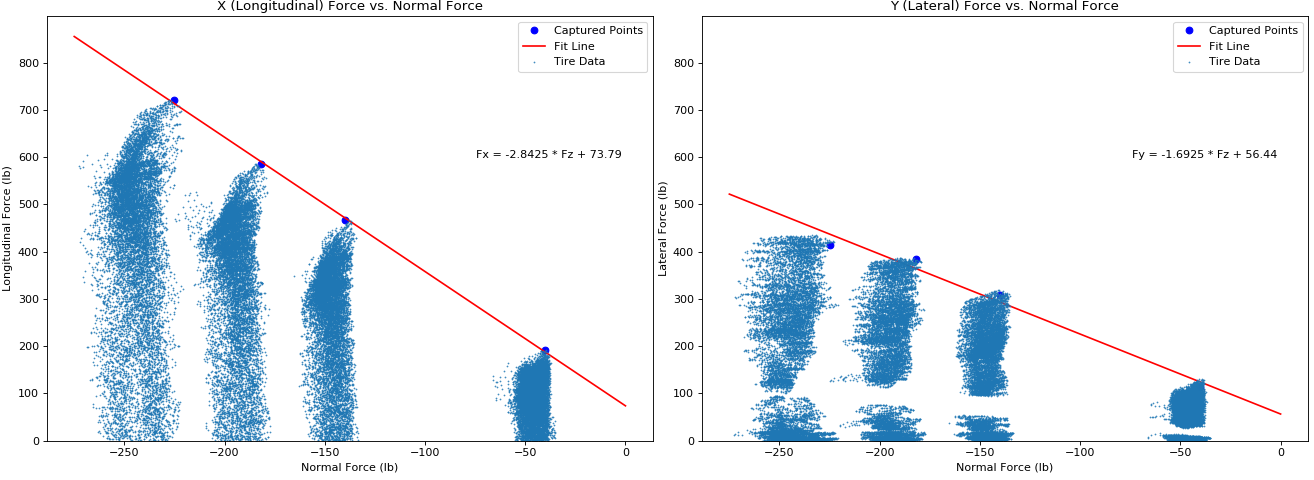
\includegraphics[width=\textwidth]{fric_regression.png}

This provides us with the four parameters for the tire: the offset and slope, in both x- and y- directions. This model is then overlaid onto the Fx-Fy data from before for comparison.

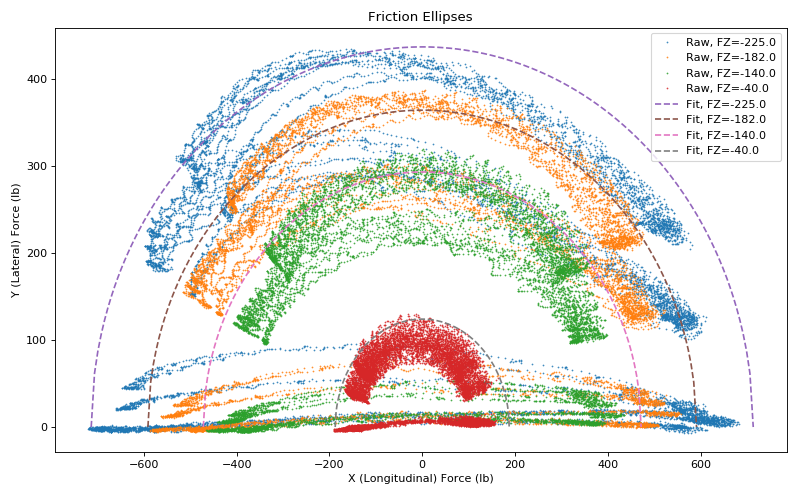
\includegraphics[width=\textwidth]{fric_ellipses_fit.png}

User adjustments can be made by changing confidence intervals, bins, or even overriding the regression results and using the charts to produce a linear fit.

\section{Component Models}

\subsection{Tires}

Tire models are extremely complicated if they are to be accurate- but this complexity can be a distraction from the major characteristics of tires that concern us. This behavior is that tires do not have a constant coefficient of friction- it decreases with additional normal force. Alternatively, we can model the tires as having some baseline, or 'offset' grip at zero normal force, and as normal force increases, maximum grip increases linearly.

\begin{align}
	F_{tire,max,lat} = F_{tire,offset,lat} + \mu_{tire,lat} N \\
	F_{tire,max,long} = F_{tire,offset,long} + \mu_{tire,long} N
\end{align}

The parameters here are only for one tire. If we wish to look at the lumped characteristics of multiple tires, we will need to do some simple division, and at the end of it all, multiply by the number of tires.

\begin{align}
	F_{tire,max,lat} = F_{tire,offset,lat} + \mu_{tire,lat} \frac{N}{n_{tires}} \\
	F_{tire,max,long} = F_{tire,offset,long} + \mu_{tire,long} \frac{N}{n_{tires}}
\end{align}

The parameters ($\mu$ and $F_{tire,offset}$) can be found from experimental tire data for various tires. The easiest method is to find lines that meet the outer capabilities of the tires, which will be at optimal operating conditions (camber, toe, slip rate, slip angle, and temperature).

Of course, a racecar tire is rarely purely in one of these conditions- we must determine the limits in a multi-axis loading. At a given normal force, a 'friction ellipse' can be produced that intercepts these limits. This can be written as

\begin{align}
	\frac{F_{tire,lat}^2}{F_{tire,max,lat}^2} + \frac{F_{tire,long}^2}{F_{tire,max,long}^2} <= 1
\end{align}

We can solve, then, for the 'remaining' lateral or longitudinal force given the other (this is still for one tire, but the lateral force is for the vehicle as a whole).

\begin{align}
	F_{tire,remaining,long} = F_{tire,max,long} \sqrt{1-(\frac{F_{tire,lateral}}{n_{tires} F_{tire,max,lat}})^2} 
\end{align}

\subsection{Aerodynamics}

Aerodynamic forces on the vehicle obey a square law relationship:

\begin{align}
	F_{down} = \alpha_{down} v^2, \\
	F_{drag} = \alpha_{down} v^2, \\
\end{align}

where $\alpha$'s are scaling constants computed from the aerodynamic forces at 35 miles per hour:

\begin{align}
	\alpha = \frac{F_{35 MPH}}{(35 MPH)^2}
\end{align}

The drag and downforce can be defined for three different aerodynamic 'modes': Full, Drag-Reduced (acceleration), and Airbrake (braking).

\subsection{Powertrain}

The force developed by the powertrain at the tires is modeled as a function of vehicle velocity and current gear.

\begin{align}
	\omega_{crank} = \frac{v}{r_{tire}} N_{final} N_{transmission,i_{gear}}, \\
	F_{long,engine,limit} = T_{engine}(\omega_{crank}) N_{final} N_{transmission,i_{gear}},
\end{align}

Where $N$ is a gear ratio, $i_{gear}$ is the gear number, and $\omega_{crank}$ is the angular velocity of the crankshaft. $T_{engine}$ is a linear interpolation representing the torque curve of the engine. For velocities that cause the engine to hit its 'rev limiter', the engine is modeled as producing zero power. For velocities that are below the lowest datapoint specified in the torque curve, the engine is modeled as producing the torque at the lowest specified RPM.

It takes a finite amount of time, $t_shift$ in order for a shift to occur. During this time, the powertrain produces no power. Another gear is chosen with a different gear than the currently selected one will yield a higher $F_{tire}$. When this happens, the driver shifts in the direction of this gear (the transmission is sequential, not fully manual). When the vehicle brakes, the gear is 'reset', and when the powertrain is used again, the best available gear is used, regardless of what was engaged prior.

\subsection{Driver}

The driver we assume (with some noted exceptions) is one which seeks to follow the ideal that racing is about maximizing acceleration in the correct direction. They use all available tire grip or engine power whenever possible, and brake as late and hard as possible. This driver does not exist in reality, but is a useful model allowing us to push the bounds for what the car can be driven to.

\subsection{Code Implementation}
These physics which are reused throughout different overall vehicle models are implemented in \texttt{vehicle.py}, which defines the \texttt{Vehicle} object type which contains methods to access this physics and has the attributes of the vehicle. Explanation of implementation is relatively straightforward and is left to the documentation in this file.

\section{Single-Tire, Point-Mass Model}

\subsection{Physics}

The physics behind a racecar are rather complicated. However, they can be simplified with the point mass assumption. This is the assumption that the car acts as a single point where all loads are applied, with no suspension to complicate tire grip and steering or tire characteristics.

Now, we can begin the vehicle physics. The forces in the vertical direction, with no vertical acceleration (I.E. perfectly flat ground) are:

\begin{align}
    -F_{down} -m g + N = m a_{z} = 0, \\
    N = m g + F_{down} \label{eq_z}
\end{align}

where $m$ is the vehicle mass, $g$ is the local acceleration due to gravity, and $N$ is the normal force of the track on the tires.

Given a specific vehicle path, we will prescribe a curvature the vehicle must pass through. The sum of forces in the lateral direction is, then,

\begin{align}
    \Sigma F_{lat} = m a_{lat} \\
    F_{tire,lat} = m v^2 k, \label{eq_lateral}
\end{align}

where $a_{lat}$ is lateral acceleration, $v$ is instantaneous vehicle velocity, and $k$ is curvature.

%By combining Equations \ref{eq_tire} and \ref{eq_lateral}, we can determine that the remaining longitudinal tire grip is:

%\begin{align}  
%    \Sigma F_{lateral} = m a_{lateral} \\
%    F_{tire,long,available} = \sqrt{ (\mu N)^2 - (m v^2 k)^2}, \label{eq_lateral}
%\end{align}
%
%Now, it is evident that we may not have remaining tire grip depending on velocity! As such, we will have to deal with going too fast later on- braking is a task that is not so straightforward.

The longitudinal forces acting on the vehicle are that of the tire and drag:

\begin{align}
    a_{longitudinal} = \frac{\Sigma F_{longitudinal}}{m}\\
    a_{longitudinal} = \frac{F_{long,tire} - F_{drag} }{m} \label{eq_accel}
\end{align}

The force of the tire, though, can vary. In the case of braking, we assume the driver has the ability to lock up the tires, but does not; i.e., the tires apply all remaining grip: 
\begin{align}
F_{long,tire,braking} = -F_{tire,long,remaining}. \label{eq_accel_brake}
\end{align}

Acceleration, though, is more complicated, as the vehicle could be limited by either tire grip or engine power:

\begin{align}
	F_{long,tire,accel} = min(F_{tire,long,remaining}, F_{engine,limit})
\end{align}

\subsection{Code Implementation and Solver}

\section{Dual-Tire, Point-Mass Model}

\subsection{Physics}

A slight improvement can be made by accounting for the longitudinal load transfer induced by acceleration and heave of the vehicle. This enables us to study the effect of center-of-gravity (CG) and center-of-pressure (CP) locations, as well as brake biasing, and any other parameter that would effect or be effected by longitudinal load transfer.

The vehicle physics begin with the summation of forces and moments in the vertical, longitudinal, and lateral directions.

\begin{align}
	\Sigma F_{vert} = N_{f} + N_{r} - m g - F_{down}(v_0) = m a_{vert} = 0 \\
	\Sigma F_{lat}  = F_{tire,lat,f} + F_{tire,lat,f} = m a_{lat} = m v^2 k \\
	\Sigma F_{long} = F_{tire,long,f} + F_{tire,long,f} - F_{drag}(v_0) = m a_{long} \\	
	\Sigma M_{vert} = F_{tire,lat,f} l_{wheelbase} = m a_{lat} l_{CG} = m v^2 k l_{CG}\\
	\Sigma M_{lat}  = N_{f} l_{wheelbase} + F_{drag}(v_0) h_{CP} - F_{down}(v_0) l_{CP} - m g l_{CG} = m a_{long} h_{CG}
\end{align}

where subscripts $f$ denote relation to the front tires, and $r$ denote relation to the rear tires. $l{CG}$ and $l_{CP}$ are the longitudinal distance from the rear tires to the CG and CP, respectively. $h_{CG}$ and $h_{CP}$ are the vertical height from the ground to the CG and CP, respectively. $l_{wheelbase}$ is the distance from the rear to front tires.

It should be noted that the summation of forces about the longitudinal axis results in the inertial force of the vehicle being the only thing to produce a moment, and as such, this is ignored, understanding that lateral load transfer is not modeled by this set of equations.

Solution of this is somewhat ugly, and most importantly, cannot be done explicitly. As such, the solution is attempted at first in a marginal fashion; this will be discussed later.

\subsection{The Marginal Physics}
This method begins by computing the required lateral force for each tire. $N_f, N_r, v0$ are presumed to be known from the previous iteration.

\begin{align}
	F_{tire,lat,f} = \frac{l_{CG}}{l_{wheelbase}} m v^2 k \\ 
	F_{tire,lat,r} = (1-\frac{l_{CG}}{l_{wheelbase}}) m v^2 k
\end{align}

The remaining longitudinal forces $F_{tire,remaining,long}$ are computed as discussed previously (normal forces are presumed to be known). 

Two models of braking may be employed: perfect brake biasing, and fixed brake biasing. Perfect brake biasing is simple:

\begin{align}
	F_{tire,long,f} = -F_{tire,remaining,long,f} \\
	F_{tire,long,r} = -F_{tire,remaining,long,r}
\end{align}

Fixed brake biasing is less so. First, the maximum total braking force must be found:

\begin{align}
	F_{brake} = min(\frac{F_{tire,remaining,long,f}}{X_{f}}, \frac{F_{tire,remaining,long,r}}{X_{r}}),
\end{align}

where $X$ is the brake bias for the front or rear tires ($X_f + X_r = 1$). Then, the brake force can be applied to the front and rear tires in the corresponding amount:

\begin{align}
	F_{tire,long,f} = - F_{brake} X_{f} \\
	F_{tire,long,r} = - F_{brake} X_{r}
\end{align}

Acceleration is the same as the point-mass model, but it is important to note that the rear-wheel tires are considered; assuming RWD rather than FWD or AWD. The overall longitudinal force, longitudinal acceleration, and final velocity can then be computed.

\begin{align}
	\Sigma F_{longitudinal} = F_{tire,long,f} + F_{tire,long,r} - F_{drag}(v_0) \\
	a_{long} = \frac{ F_{tire,long,f} + F_{tire,long,r} - F_{drag}(v_0)}{m} \\
	v_{final} = \sqrt(v_0^2 + 2 a_{long} x_{segment}
\end{align}

\subsection{Working Backwards}
This method determines the forces on the vehicle given a prescribed $a_{long}$.

The normal forces on the tires can be found by solving the summation of forces in the and vertical direction, and summation of moments about the lateral axis. This results in:

\begin{align}
	% Big gross equations, dump em here
\end{align}

The required lateral forces from the tires are also computed:

\begin{align}
	F_{tire,lat,f} = \frac{l_{CG}}{l_{wheelbase}} m v^2 k \\ 
	F_{tire,lat,r} = (1-\frac{l_{CG}}{l_{wheelbase}}) m v^2 k
\end{align}

From here, the remaining longitudinal tire grip can be computed.
\begin{align}
	F_{tire,long,total,required} = \frac{a_{long}}{m} + F_{drag}(v)
\end{align}

We must then compute the required longitudinal tire grip to maintain the desired $a_{long}$ and counteract drag. For the acceleration case, this is straightforward:

\begin{align}
	F_{tire,long,r,required} = F_{tire,long,total,required}
\end{align}

For the braking case where fixed biasing is used, the process is very simple: distribute the required force between the tires.
\begin{align}
	F_{tire,long,r,required} = F_{tire,long,total,required} X_r \\
	F_{tire,long,f,required} = F_{tire,long,total,required} X_f
\end{align}

For the braking case where perfect biasing is used, this requires some thinking. Since in this model, the front and rear braking forces are colinear, it makes no difference to where the braking force is distributed (provided that the maximum grip is not exceeded). We will use up all of the rear tire's grip before using the front tire's grip.

\begin{align}
	F_{tire,long,r,required} = F_{tire,long,total,required} \\
	if F_{tire,long,remaining,r} < F_{tire,long,r,required} \\
		F_{tire,long,remaining,f} = F_{tire,long,total,required} - F_{tire,long,r,required}
\end{align}

From here, checks may be performed to ensure that grip is used appropriately, and final velocity is calculated much like before.

\subsection{Code Implementation and Solver}

\section{Point Simulations}

\subsection{Competition Formulae}

\subsection{Code Implementation}

\section{Post-Processing}

\section{Future Plans}
Write your conclusion here.

Tire temps would be interesting???
CVTs maybe yo

\end{document}
